% FIG ch02-06 NMC final overlay (English) — requires codex base image
\begin{tikzpicture}
  \node[anchor=south west, inner sep=0] (img) at (0,0)
    {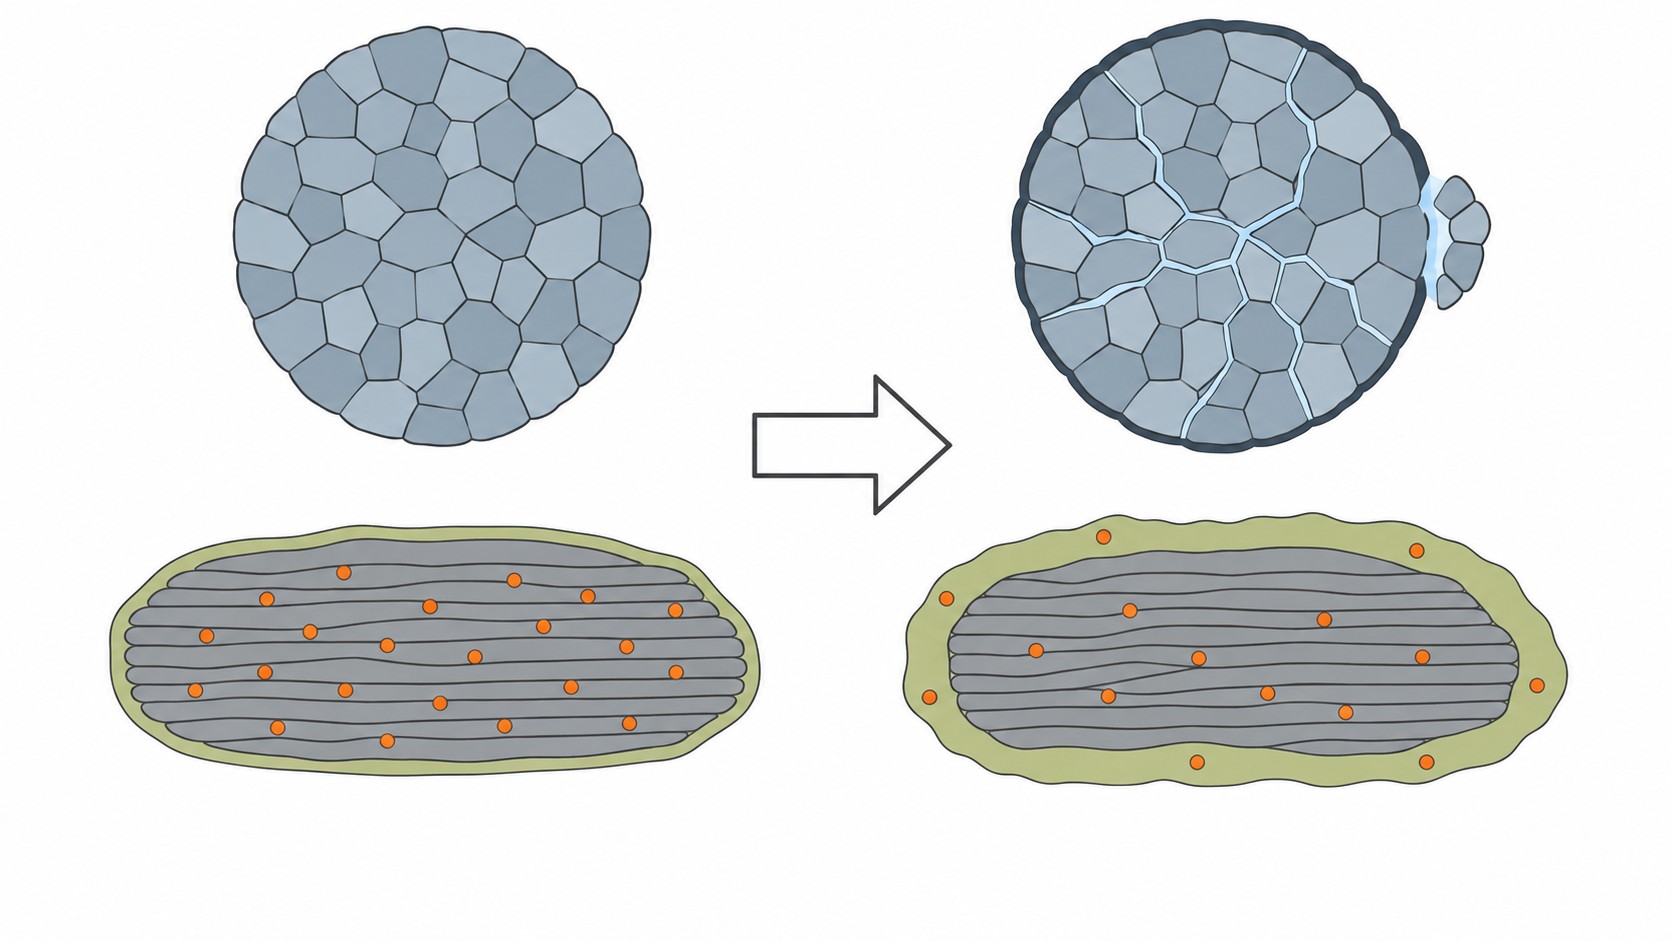
\includegraphics[width=\linewidth]{figures/ch02/ch02-06-nmc-v3-base.png}};
  \begin{scope}[x={(img.south east)}, y={(img.north west)},
    font=\sffamily\fontsize{7}{8}\selectfont]
    \node[font=\bfseries] at (0.25, 0.96) {Pristine};
    \node[font=\bfseries] at (0.75, 0.96) {After cycling};
    \node[align=center, anchor=west] at (0.04, 0.70) {NMC\\secondary\\particle};
    \node[anchor=west] at (0.04, 0.30) {Graphite anode};
    \node at (0.50, 0.58) {Cycling};
    \node[anchor=west] at (0.14, 0.86) {Primary grains};
    \draw[BookInk!40, thin] (0.14, 0.84) -- (0.18, 0.82);
    \node[anchor=west, align=left] at (0.66, 0.88) {Intergranular cracks\\(electrolyte ingress)};
    \draw[BookInk!40, thin] (0.66, 0.86) -- (0.58, 0.84);
    \node[draw=BookInk, line width=0.4pt, fill=white, fill opacity=0.85, text opacity=1,
      align=left, inner sep=2pt, anchor=west] at (0.90, 0.80)
      {Reconstructed surface layer\\→ higher impedance};
    \node[draw=BookInk, line width=0.4pt, fill=white, fill opacity=0.85, text opacity=1,
      align=left, inner sep=2pt, anchor=west] at (0.90, 0.62)
      {Detached fragment\\→ loss of active material};
    \node[draw=BookInk, line width=0.4pt, dashed, fill=white, fill opacity=0.85, text opacity=1,
      align=left, inner sep=2pt, anchor=west] at (0.66, 0.52)
      {Side reactions on new crack surfaces\\→ higher impedance (hypothesis)};
    \node[anchor=west] at (0.12, 0.18) {SEI};
    \draw[BookInk!40, thin] (0.12, 0.20) -- (0.16, 0.22);
    \node[draw=BookInk, line width=0.4pt, fill=white, fill opacity=0.85, text opacity=1,
      align=left, inner sep=2pt, anchor=west] at (0.86, 0.22)
      {Thicker SEI\\→ loss of cyclable lithium};
  \end{scope}
  \begin{scope}[x={(img.south east)}, y={(img.north west)},
    font=\sffamily\scriptsize]
    \node[align=center] at (0.50, 0.05) {%
      Legend: solid box = established; dashed box = authors' hypothesis; orange dots = lithium (schematic)};
  \end{scope}
\end{tikzpicture}
